% Resumen de una plana: Procesos de ramificación en complejos celulares
\documentclass[10pt]{article}
\usepackage[a4paper, top=1.3cm, bottom=1.3cm, left=1.5cm, right=1.5cm]{geometry}
\usepackage[T1]{fontenc}
\usepackage[utf8]{inputenc}
\usepackage[spanish,es-noshorthands,es-nodecimaldot]{babel}
\usepackage{lmodern}
\usepackage{microtype}
\usepackage{amsmath,amssymb}
\usepackage{graphicx}
\usepackage{multicol}
\usepackage{enumitem}
\usepackage{xcolor}
\usepackage[hidelinks]{hyperref}
\graphicspath{{figuras/}}

\definecolor{cafe}{HTML}{3E271C}
\definecolor{dulce}{HTML}{C4864A}
\definecolor{dulceosc}{HTML}{A0642C}

\newcommand{\Z}{\mathbb{Z}}
\DeclareMathOperator{\sgn}{sgn}
\newcommand{\ip}[2]{\langle #1,#2\rangle}
\newcommand{\seccion}[1]{\par\vspace{1.6mm}{\color{dulceosc}\bfseries\large #1}\par\vspace{0.6mm}}

\pagestyle{empty}
\setlength{\parindent}{0pt}
\setlength{\parskip}{1.1mm}
\setlength{\columnsep}{7mm}
\setlist{nosep, leftmargin=4mm, itemsep=0.6mm}
\color{cafe}

\begin{document}

{\LARGE\bfseries Procesos de ramificación en complejos celulares}\\[1mm]
{\large Simulación, extinción y conjuntos absorbentes}\\[1.5mm]
\textbf{Martín Maturana Acevedo · Bruno Guevara}\hfill{\small Simulación Estocástica · Universidad de Chile · Primavera 2026}\\[-1mm]
{\color{dulce}\rule{\textwidth}{0.8pt}}

\begin{multicols}{2}

\seccion{El modelo}
Basado en el borrador \emph{Branching process on complexes} (D.~Cid y A.~Sepúlveda). Sobre las aristas de una caja de $\Z^d$ vive una configuración $\theta\in\Z^{E}$ de partículas con signo. Cada partícula, a tasa~1 por cada cara $f$ que la contiene, se aniquila y deja partículas en el resto del borde de~$f$:
\[
  \theta\;\longmapsto\;\theta-\ip{e}{\partial f}\,\sgn(\theta_e)\,\partial f .
\]
Una partícula da lugar a tres, las cargas opuestas se cancelan y las que caen en un conjunto absorbente $T$ de aristas mueren. El generador cumple $\mathcal{L}I(\theta)=-\Delta_1^{\uparrow}\theta$, con $\Delta_1^{\uparrow}=\partial_2\partial_2^{\top}$ el Laplaciano de Hodge superior: la media sigue la ecuación del calor, $\mathbb{E}[\theta_t]=e^{-t\Delta_1^{\uparrow}}\theta_0$, y la ramificación vive en las fluctuaciones. El borrador prueba la extinción cuando $T$ es un \textbf{árbol generador}.
\begin{center}
  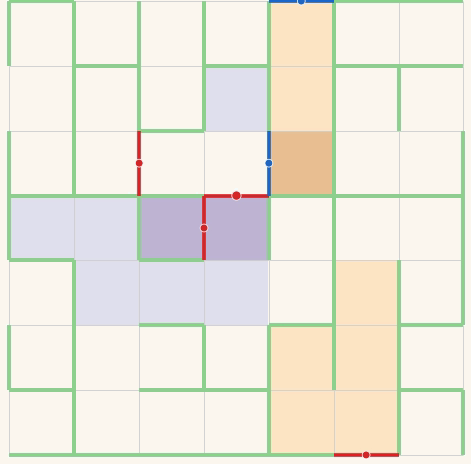
\includegraphics[height=2.8cm]{portada_2d}\hspace{5mm}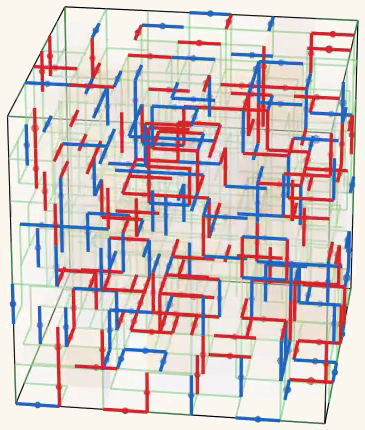
\includegraphics[height=2.8cm]{portada_3d}\\[0.3mm]
  {\footnotesize Partículas $+$ en rojo y $-$ en azul; aristas absorbentes $T$ en verde.}
\end{center}

\seccion{La pregunta}
¿Qué pasa con otros conjuntos absorbentes? ¿Cuándo es posible la extinción, con qué probabilidad y cuánto tarda, al ir agregando aristas a~$T$?

\seccion{Método}
\begin{itemize}
  \item Celdas como puntos de $(\tfrac12\Z)^d$ ($k$ coordenadas semienteras) y operadores $\partial_k$ como matrices dispersas, en cualquier dimensión.
  \item \textbf{Gillespie exacto} en tiempo continuo: el reloj total es $\mathrm{Exp}\big(\sum_e|\theta_e|\lambda_e\big)$ y cada evento toca 4 aristas ($\sim\!10\,\mu$s por evento).
  \item Miles de réplicas en paralelo con semillas independientes; proporciones con intervalos de \textbf{Wilson} al 95\,\%.
  \item Verificado contra la teoría: la deriva estimada coincide con $-\Delta_1^{\uparrow}\theta$ (error de 0.55\,\%) y la cota de Lyapunov del borrador se cumple.
  \item Sin selección de trayectorias: se usa la primera semilla y se corre hasta la extinción.
\end{itemize}

\seccion{Resultados}
\textbf{1. Cargas conservadas.} Para cada componente $C$ del grafo $(V,T)$, la carga $Q_C=\sum_{v\in C}(\partial_1\theta)(v)$ no cambia en ningún evento. Si alguna es no nula, la extinción es \emph{imposible}; si todas son nulas, el argumento de Lyapunov del borrador da extinción casi segura (bajo una hipótesis de accesibilidad que las simulaciones respaldan). Coincide réplica a réplica en 2400 simulaciones (fig.~a).

\textbf{2. Extinción eventual exacta.} Con las cargas, $\mathbb{P}(\tau<\infty)$ es un problema de conectividad del grafo aleatorio $(V,T)$, tipo percolación: se calcula exactamente con union-find y es \emph{monótona} en~$T$. En $9\times9$, con 99 aristas absorbentes (las de un árbol generador), diez partículas se extinguen con probabilidad 0.31 si las aristas son uniformes y con probabilidad~1 si forman un árbol aleatorio (fig.~b). El lazo $\partial f$ se extingue con cualquier~$T$.

\textbf{3. La velocidad no es monótona.} Para el lazo, agregar aristas absorbentes \emph{retrasa} la extinción: $\mathbb{P}(\tau\le50)$ baja de 1.00 a 0.94 con el árbol completo (fig.~c), porque absorber corta el lazo en cadenas abiertas que ya no se aniquilan solas. Si $T$ crece durante la simulación, crecer rápido acelera la extinción de una partícula ($\mathbb{E}[\tau]$: 69 frente a 432) y retrasa la del lazo (9.7 frente a 1.1).

\textbf{4. En 3D aparece una meseta.} Aun con extinción segura, el proceso queda en un régimen cuasi-estacionario de cientos de partículas. En $3\times3\times3$ la extinción tardó 23 y 90 millones de eventos, con una caída final brusca.

\seccion{Preguntas abiertas}
Demostrar la hipótesis de accesibilidad; la conjetura $\gamma(T)\approx\lambda_{\min}\big(\Delta_1^{\uparrow}|_{E\setminus T}\big)$ para la tasa de extinción con árbol fijo (correlación 0.95 en 40 árboles); explicar la no monotonía; estudiar la meseta con Fleming--Viot.

\end{multicols}

\vspace{-1mm}
\begin{center}
  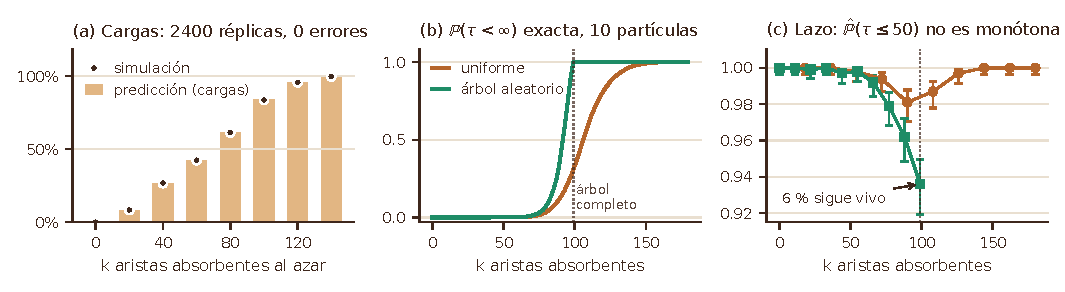
\includegraphics[width=\textwidth]{resultados}
\end{center}
\vspace{-3mm}
{\small Caja $9\times9$. (a) Barras: réplicas en que las cargas permiten la extinción; puntos: réplicas que se extinguieron. (b) Probabilidad exacta de extinción eventual de 10 partículas según la regla para agregar aristas. (c) Probabilidad de que el lazo se extinga antes de $t=50$ (colores como en b), 1000 réplicas por punto, con intervalos de Wilson.}

\vfill
{\color{dulce}\rule{\textwidth}{0.5pt}}\\
{\small Código, videos y documento de explicación: \url{https://github.com/martinmaturana777/Branching-Process-Complexes}}

\end{document}
